%%
%% THIS IS THE LaTeX RESEARCH PLAN TEMPLATE OF THE RESEARCH COUNCIL OF FINLAND FOR THE 2026 INTERNATIONAL COLLABORATION IN HIGH-PERFORMANCE COMPUTING CALL.
%%
%% THE STYLE AND HEADERS HAVE BEEN PRESET ACCORDING TO THE RESEARCH COUNCIL'S RULES. THE RESULTING PDF FILE OF THE RESEARCH PLAN WILL BE AUTOMATICALLY CHECKED WHEN UPLOADING IT. THE APPLICATION CANNOT BE SUBMITTED IF THE SYSTEM DETECTS AN DEVIATION IN THE HEADINGS, THE PAGE CONFIGURATION OR THE STRUCTURE OF YOUR RESEARCH PLAN PDF FILE.
%%
%%
\documentclass[a4paper,12pt]{article}

% Language support (including nordic letters)
\usepackage[T1]{fontenc}
\usepackage[english]{babel}

% Math support
\usepackage[intlimits]{amsmath}
\usepackage{amsthm}
\usepackage[sort&compress]{natbib}
    \bibliographystyle{aasjournal}

% Symbol support
\usepackage{amssymb}
\usepackage{eurosym}

% Image support and enabling wrapping of images
\usepackage[pdftex]{graphicx}
%\usepackage{wrapfig}

% Table extras support and using colors
\usepackage[table]{xcolor}
%\usepackage{booktabs}

% Item list extras for reduced spacing between items
\usepackage{enumitem}
\setlist{nosep}

% Hyperlink support (only for external hyperlinks)
\usepackage[implicit=false]{hyperref}
\hypersetup{
    colorlinks=true,
    urlcolor=cyan,
}
\usepackage[most]{tcolorbox} % Required for boxes that split across pages
\usepackage{tabto}
\usepackage{multicol}
\usepackage[font=small]{caption}
\newcommand{\NO}{{\textsf{NO}}}
\newcommand{\BO}{{\textsf{BO}}}
\newcommand{\NL}{{\textsf{NL}}}
\newcommand{\BL}{{\textsf{BL}}}
\newcommand{\NH}{{\textsf{NM}}}
\newcommand{\BH}{{\textsf{BM}}}

\definecolor{yellow}{RGB}{252, 211, 3}
\definecolor{green}{RGB}{60,179,113}
\definecolor{blue}{RGB}{3, 165, 252}
\definecolor{midblue}{rgb}{0.0,0.4,0.7}
\definecolor{midgreen}{rgb}{0.1,0.6,0.3}
\definecolor{mypurple}{rgb}{0.7,0.3,0.8}
\newcommand{\fg}[1]{\textcolor{midblue}{#1}}
\newcommand{\fag}[1]{\textcolor{midblue}{[FAG: #1]}}
\newcommand{\lm}[1]{\textcolor{mypurple}{#1}}
\newcommand{\lars}[1]{\textcolor{mypurple}{[LM: #1]}}
\newcommand{\wpdef}[3]{\hypertarget{wp#1}{\subsubsection*{WP#1 {\normalfont(#2)}: #3}}}
\newcommand{\wpref}[1]{\protect\hyperlink{wp#1}{\textbf{WP#1}}}

\usepackage{pgfgantt}
\ganttset{canvas/.append style={fill=none, draw=black!10, line width=1pt},
    hgrid style/.style={draw=black!5, line width=.75pt},
    vgrid={*1{draw=black!10, line width=1pt}},
    title/.style={draw=none, fill=none},
    title label font=\bfseries\footnotesize,
    y unit title=0.5cm,
    title height=1,
    include title in canvas=false,
    bar label font=\mdseries\footnotesize\color{black!70},
    bar/.append style={draw=none, fill=blue, opacity=0.4},
    group/.append style={draw=none, fill=blue},
    group left shift=0,
    group right shift=0,
    group height=.5,
    group peaks tip position=0,
    y unit chart=0.5cm,
    x unit=0.57cm,
    link/.style={-latex, rounded corners=1pt, black!63},
    link label font=\footnotesize\bfseries,
    link label node/.append style={below left=-2pt and 0pt},
    milestone label font=\footnotesize,
    group label font=\footnotesize\bfseries,
}
%% N.B. YOU MAY ALSO ADD YOUR OWN LaTeX PACKAGES HERE. NOTE THAT THE PACKAGES CANNOT BE IN CONFLICT WITH OR OVERRUN THE TEMPLATE SETTINGS SET BY THE RESEARCH COUNCIL OF FINLAND.

%-----------------------------------------------------
% RESEARCH COUNCIL SETTINGS: DO NOT ALTER THESE SETTINGS!
%-----------------------------------------------------

% Instruction text definition.
\newcommand{\instructions}[1]{\textcolor{blue}{#1}}

\newcommand{\mnras}{MNRAS}
\newcommand{\apj}{ApJ}
\newcommand{\apjs}{Ap\&SS}
\newcommand{\apjl}{ApJl}
\newcommand{\aap}{A\&A}
\newcommand{\araa}{ARA\&A}
\newcommand{\prl}{Phys.\,Rev.\,Let.}
\newcommand{\jcap}{JCAP}

\newcommand{\answer}[1]{
	\begin{tcolorbox}[breakable, enhanced, colback=pink]
		#1
	\end{tcolorbox}
}

% ONLY CALIBRI/CARLITO ARE ALLOWED AS FONT, FONT SIZE 12 PT DEFINED ABOVE. The font is used to ensure equal settings between LaTeX and Word templates.
% Find the font package here: https://www.ctan.org/tex-archive/fonts/carlito
\usepackage[sfdefault]{carlito}

% Linespacing 1 support and set space
\usepackage{setspace}
\singlespacing

% Page margin support and set page margins 20 mm
\usepackage[left=20mm, top=20mm, bottom=20mm, right=20mm]{geometry}

% Setting spacing for section, subsection and paragraph
\usepackage{titlesec}
\titleformat*{\section}{\large\bfseries}
\titleformat*{\subsection}{\bfseries}
\titlespacing{\section}{0 cm}{6pt}{0pt}
\titlespacing{\subsection}{0 cm}{6pt}{0pt}
\setlength{\parskip}{6pt}

%Aligning text to left
\raggedright

% Sets page numbers and header
\usepackage{fancyhdr}
\pagestyle{fancyplain}
\fancyfoot{}
\fancyhead{}
\renewcommand{\headrulewidth}{0pt}
\rhead{\fancyplain{}{\thepage}({\pageref{lastpage}}) }

%-----------------------------------------------------

%%%%%%%%%%%%%%%%%%%%%%%%%%%%%%%%%%%%

\begin{document}

%% GENERAL INFORMATION REGARDING THE RESEARCH PLAN.
%% Please compile before starting for the instructions to be visible in the pdf file.
%% The instructions environments should be deleted when preparing your text.

\instructions{
\textbf{\Large{2026 International collaboration in high-performance computing: Guidelines and template for research plan}}\\
\vspace{10pt}
The research plan is submitted as a PDF appendix on the tab ‘Research plan’ in the online services. Remember to convert the file into PDF  format before attaching it in the application form. Name the attachment file as follows: \textbf{Research\_plan\_yoursurname.pdf}. \\
\vspace{10pt}
%
Read the \href{https://www.aka.fi/en/research-funding/apply-for-funding/calls-for-applications/}{call text} carefully and familiarise yourself with the \href{https://www.aka.fi/en/research-funding/peer-review-and-funding-decision/guides-for-reviewers/}{review guidelines, review form and principles of responsible evaluation} before you start writing the plan.
%
\begin{itemize}
    \item The maximum length of the research plan is 12 pages.
    \item The maximum length of a consortium research plan is 15 pages.
    \item The paper size is A4.
    \item The font is Calibri/Carlito 12 pt.
    \item The line spacing is 1.
    \item The margins are 20 mm.
    \item The text is left-aligned.
    \item Do not use paragraph indents.
    \item The font size in tables and images must be at least 10 pt.
    \item Use a single-column layout when writing the text.
    \item The list of references is included in the length of the research plan. The font size in the list is 10 pt.
    \item All references must be added directly into the text, for example as follows: (author(s), year) or [number]. You must not use footnotes.
    \item The maximum size of the PDF appendix is 50 MB.
\end{itemize}
%
\textbf{The instructions and structure provided must be followed} to ensure the equal treatment of applicants. Use the headings provided. The application cannot be submitted if the system detects an deviation in the headings, the page configuration or the structure.
%
\begin{itemize}
    \item Write the research plan on this template.
    \item Fill in the sections according to the practices of your own discipline.
    \item You cannot edit or delete the headings in the template. If necessary, you may add subheadings.
    \item See the \href{https://www.aka.fi/en/online-services/}{How-to guides for the online services} on our website for the technical instructions.
\end{itemize}
%
Please, delete the instructions environments in blue when preparing your text.
\noindent\rule[0.5ex]{\linewidth}{1pt}
}

%% >>>>>>>>>> ADD YOUR RESEARCH PLAN TITLE IN THE FIELD BELOW:
\textbf{\LARGE{Extended multi-scale code-coupling for dust processing in supernova-driven turbulence}}\\

%% >>>>>>>>>> ADD YOUR NAME AND THE ABBREVIATION OF CONSORTIUM IF APPLICABLE:
Maarit J. Korpi-Lagg (SNDust)

%%%%%%%%%%%%%%%%%%%%%%%%%%%%%%%%%%%%

\section{Background and significance}

\instructions{
  	In this section, describe the following aspects:
    \begin{itemize}
        \item {Significance of research project in relation to current knowledge, research-based starting points}
        \begin{itemize}
            \item How the project and the methods used are linked to previous international and/or national research (state of the art)
            \item Research premise, aims and objectives
        \end{itemize}
        \item{Research questions and/or hypotheses}
        \item Special objective of call
	\begin{itemize}
		\item Justifications for how the project will address the call objectives and questions such as:
		\begin{itemize}
				\item how the use of European High-Performance Computing (EuroHPC) or the Large Unified Modern Infrastructure (LUMI) supercomputer resources is justified and will benefit the project
				\item how the project and the international collaboration within the project can contribute to the expansion of computing expertise at both national and international level
  				\end{itemize}
		\end{itemize}
    \end{itemize}
}

\fag{incorporate work of new collaborators here and expand on the scientific questionmarks/hypotheses}

\fag{add how the project justifies the use of LUMI resources}

We plan to implement groundbreaking coupled multi-tiered, or
{\textit{extended multi scale simulations}} (EMS), bridging previously
unattainable scales of separation. Extreme scales of separation are generic in astrophysics, where this innovative concept shall be applied to dust,
but our new interactive control tools would have applicability in other
disciplines proliferated by large and heterogeneous data.

A common alternative approach is \textit{adaptive mesh refinement} (AMR), in
which higher resolution meshes are dynamically applied locally where,
typically, densities exceed some threshold \cite{AMR00}.  However, in MHD the
strongest turbulence and critical dynamo action often occur in regions of high
temperatures and low densities. This does not permit solving additional physics
relevant only to the zoomed in region. Additionally, non-uniform discrete
Fourier transform that would be used to understand the spectral properties of
turbulent fields are challenging to determine \cite{NUFFT}. Multi-grid methods
are also commonly employed for improving convergence with implicit solvers of
highly non-linear systems in chemistry \cite{MGRID}, engineering and other
disciplines, with increased overheads. Our approach will use multi-grid tools to
extend the scales and physics accessible to the hierarchy of simulations with
minimal increase in overheads.

Another resource applying a common interface to multiple astrophysics is the
Astrophysical Multipurpose Software Environment \cite{AMUSE}.  Its Python
interface is relatively user friendly, but has limited scalability via parallel
high performance computation. Our project shall implement integrated highly
scalable simulations capable of handling huge data, while also developing user
friendly interactive tools with which to manage and interrogate the
applications.

Our recent breakthrough \citep{KMG24} revealed how cosmic dust, the building
blocks of planets, can survive destruction by supernovae (SNe) more than
previously thought. We showed that, relative to the commonly used uniform
interstellar medium (ISM), including a realistic in-homogeneous and turbulent
ISM can reduce 50\% the amount of ambient dust destroyed during the lifetime of
an SN remnant.  We also found that including the Lorentz force of the turbulent
magnetic field acting on the dust further halved these losses, a much greater
effect than had been anticipated.  Even larger scales are required to fully
model the magnetic field structure and yet smaller scales to properly
understand the dust processing. To advance this scientific goal we need the
multi-tiered approach and the machine-learning toolkit to facilitate
identifying critical features, launching coupled simulations and managing
communication and balancing resources within a typical HPC batch system.

%==============================================================================
\begin{figure}
\begin{minipage}[h]{0.7\textwidth}
      \resizebox{\hsize}{!}{
      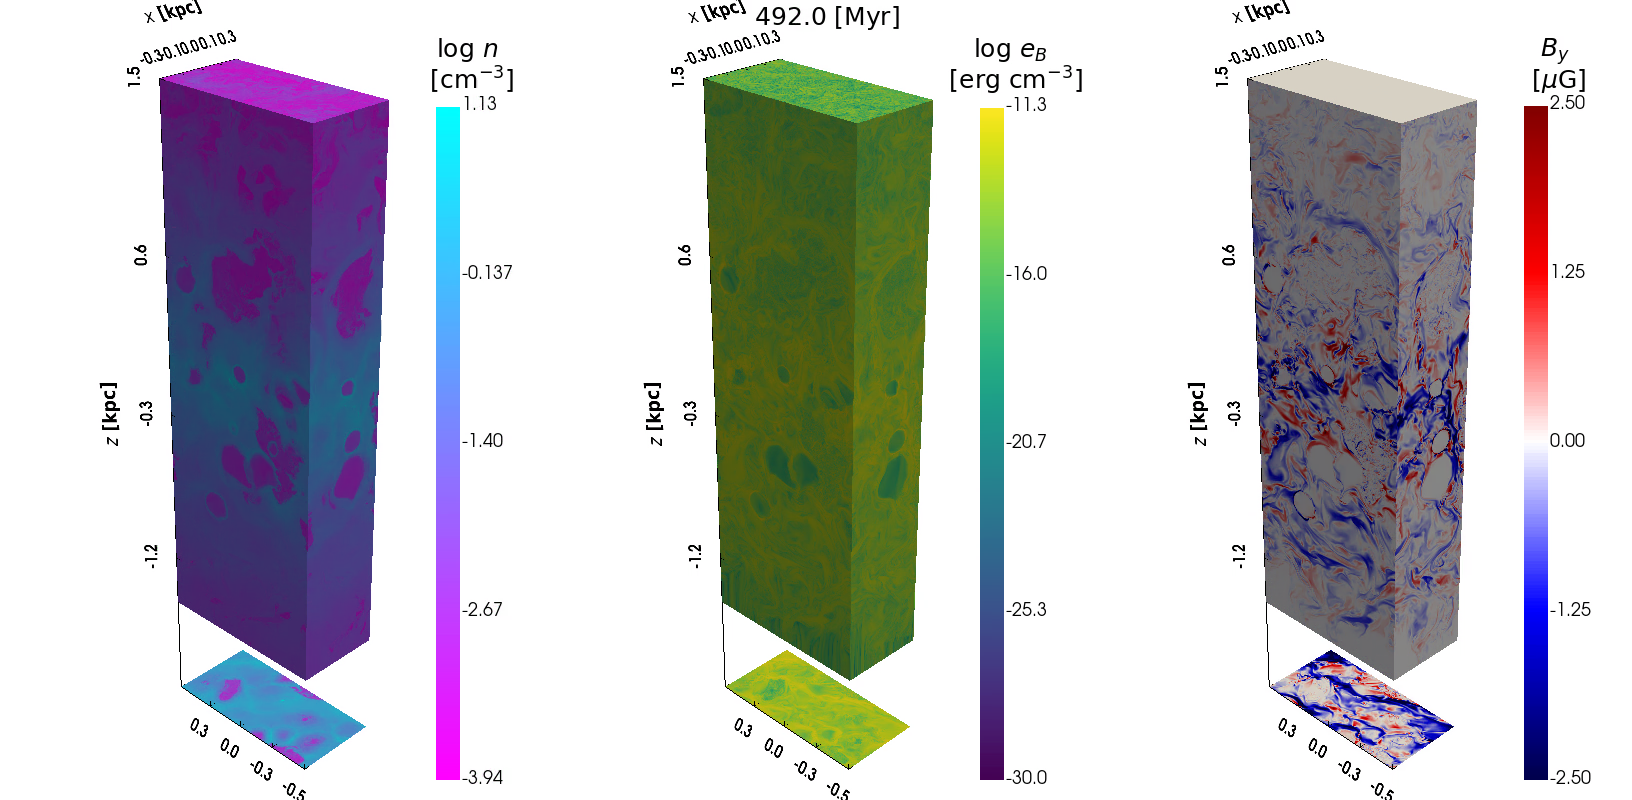
\includegraphics[trim=3.5cm 0.0cm 0.0cm 0.0cm,clip=true,height=1.18\columnwidth]{Pics/vlcsnap-2025-01-31-13h38m50s316.png}
        }
\end{minipage}
\begin{minipage}[h]{0.29\textwidth}
  \caption{\footnotesize \label{ISMsim}\label{ISMsim2} Typical snapshots of gas number $n$ and magnetic energy $e_B$ density and magnetic field $B_y$
from an MHD simulation of SN-driven turbulence and galactic dynamo
\citep{GMK24}. Turbulence drives a fast small-scale dynamo, which can create
magnetic fields within a few percent of the kinetic energy of the turbulence,
while stratification about the galactic disc regulates the multi-phase
structure of the ISM via outflows and inward precipitation. Large-scale shear
is required for a mean-field dynamo, which continues the growth of the magnetic field to energy equipartition with its kinetic energy.
}
\end{minipage}
\end{figure}
%==============================================================================

Cosmic dust plays a critical role in many astrophysical processes, a catalyst
in star and planet formation and, due to its heat absorption and light
scattering, important in galaxy evolution and multi-phase structure of the ISM.
Heavy elements are forged in stars, the heaviest metals fusing at the explosive
death of the largest stars, and thus ejected into the ISM by SNe. Some of these
form dust, comprising a mixture of carbonaceous material and silicates
\citep{Weingartner01}. The abundance or composition of dust is indicative of a
galaxy's age and star formation rate.  Although SNe eject into the ISM some
fraction of dust, their highly supersonic blast waves destroy masses of dust
already present in the ambient ISM \citep{McKee89}.  Estimates of dust
abundances in early galaxies appear too high, given prevailing models of
destruction rates and accumulation mechanisms.  This has even been considered
by some as a {\textbf{dust budget crisis}} \citep{Rowlands14b}.
Sublimation, condensation, grain-grain interactions, ion sputtering are well established as
primary dust destruction mechanisms in SN blasts \citep{Jones11}.  The
resultant dust properties are, however, highly uncertain.  Both processing and
formation of ISM dust remain poorly understood \citep{Draine09} and most models
omit realistic ISM turbulence.
%done

Simulations to sixth-order accuracy explore many scales of the ISM.  Due to a vast range
of scale in space and time all models, full galaxy or inside star-forming
molecular clouds (MC), must exclude some physics from their scope.  Models at
kpc-scale (see, e.g., Figure~\ref{ISMsim}) of SN-driven turbulence on
stratified discs with galactic-shear dynamo \citep[e.g.,][]{
GMK24} omit dust processing, but acquire the
necessary turbulent structure.  Dust would decouple from the gas
\citep[][]{Mattsson18a} and, because grains are easily charged, radiation
pressure and Lorentz forces affect its critical MC scale distribution.

To bridge the gap between scales relevant to dust processing and the numerical
scales required to model the realistic multi-phase turbulent ISM, we have
treated dust as a distribution of multiple fluids binned by grain size and
applied onto prior MHD data \textsc{Paperboats} \citep{Kirchschlager19}. Our
breakthrough results \citep{KMG24} applied \textsc{Paperboats} to process dust
on 2D slices taken from the 3D MHD \textsc{Pencil Code} \citep{Pencil-Joss}
model of turbulent SN-driven dynamo \citep{GMKS21, GMKS22}.  As illustrated in
Figure~\ref{fig_gsd} the magnetic field has a more significant effect on dust
resilience than might be expected above that offered by turbulence.  A
comprehensive review of MHD simulations at multiple scales \citep{Whitworth24},
exploring correlations between gas number density $n$ and magnetic field
strength $B$, conclude \citet{GMK24} obtained $B-n$ relations which are among
the best match to those from observations.  Large scale dynamo (LSD) and a
realistic multi-phase ISM are thus critical ingredients.
%done

\begin{minipage}[h]{0.6\textwidth}
 \begin{center}
%\begin{figure}
 %\resizebox{0.9\hsize}{!}{\hspace*{-0.6cm}
 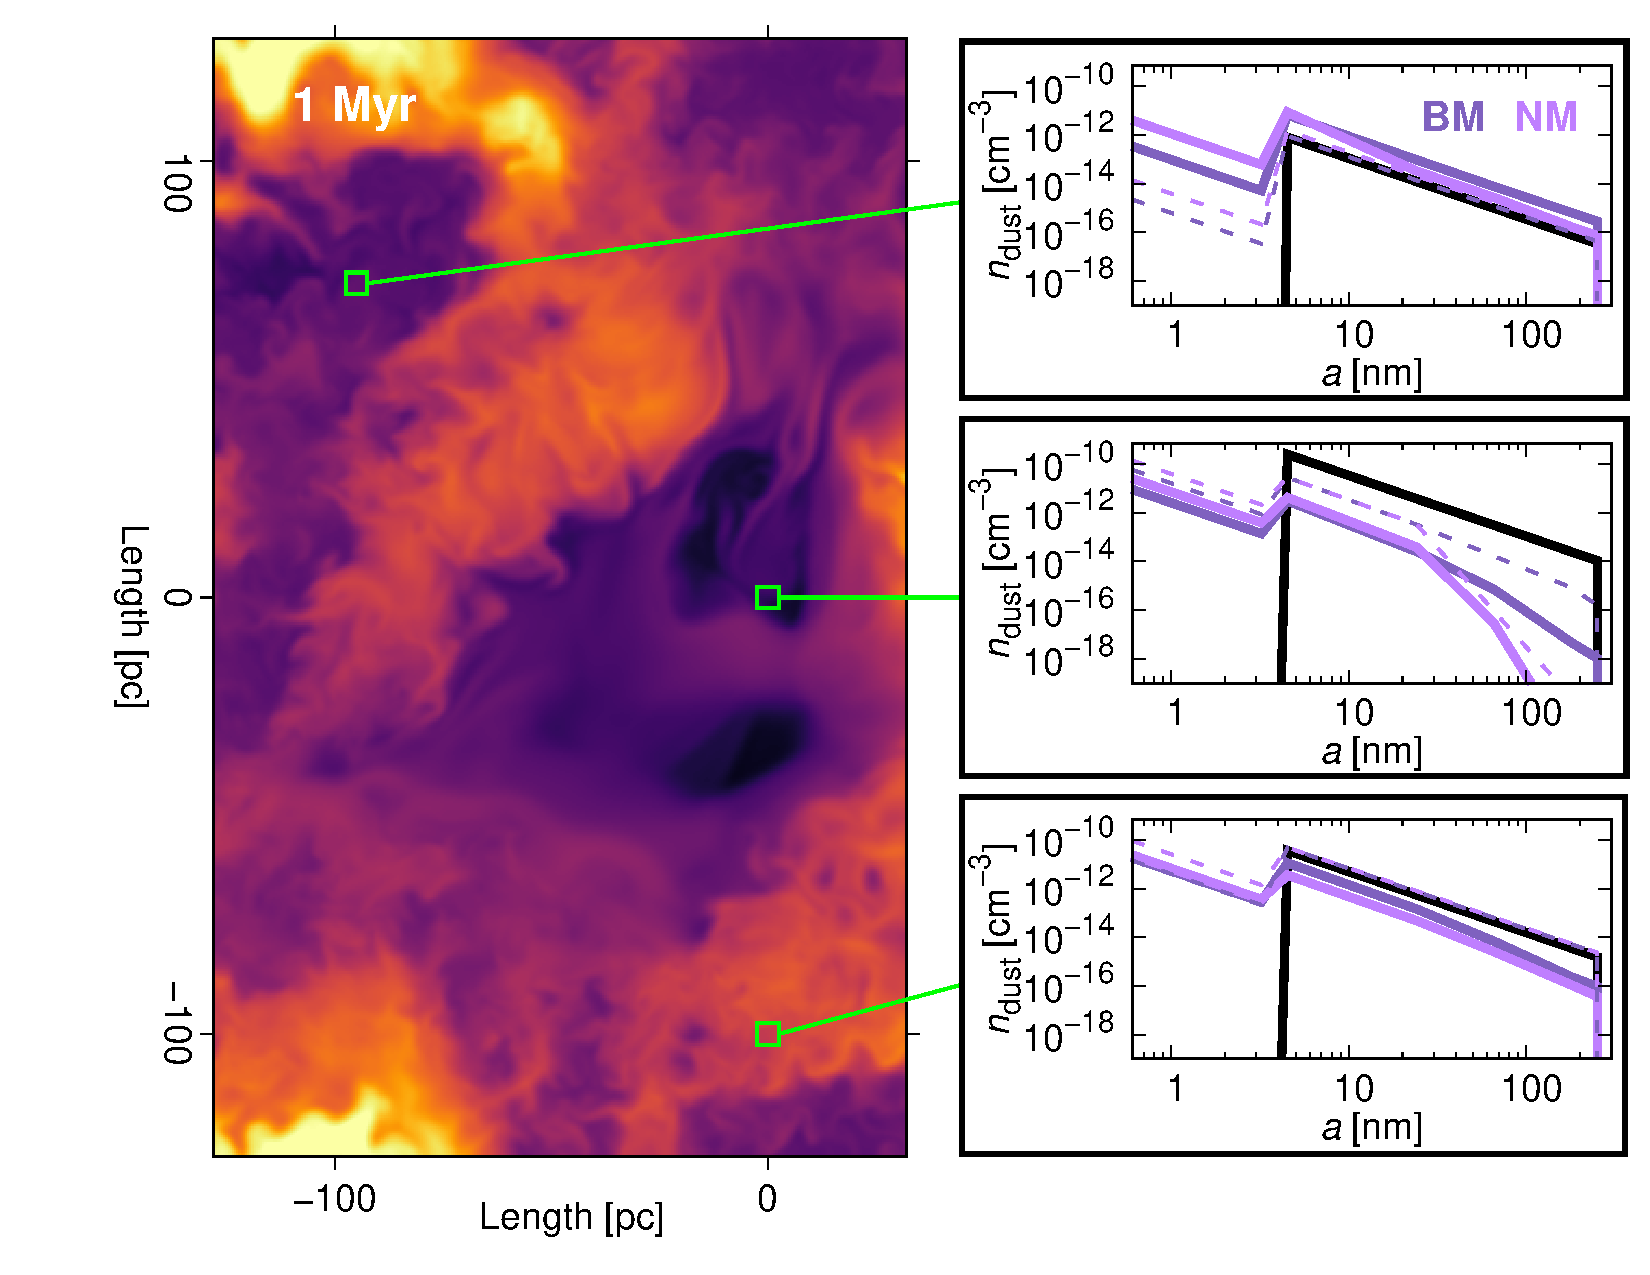
\includegraphics[trim=1.9cm 0.6cm 0.35cm 0.2cm,  clip=true, width=\textwidth]{Pics/GrainSizes_04000_800Edi.pdf}
 %}
 \begin{picture}(0,0)
    \put(-139,232){\footnotesize(\textbf{\textsf{a}})}
    \put(   6,232){\footnotesize(\textbf{\textsf{b}})}
    \put(   6,166){\footnotesize(\textbf{\textsf{c}})}
    \put(   6, 90){\footnotesize(\textbf{\textsf{d}})}
  \end{picture}
 \end{center}
 \end{minipage}
\quad
\begin{minipage}[h]{0.37\textwidth}
%\vspace{-1cm}
  \captionof{figure}{Regional variation of dust distribution at sampled times.
({\textbf{a}}) Location of three specimen regions (green boxes) in the vicinity
of an SN blast wave, each of size of $5\, \text{pc}\times5\, $pc.  Dust
distributions ({\textbf{c}}) about the SN center, and ({\textbf{b}}) and
({\textbf{d}}) at unshocked diffuse or moderate density regions, respectively.
Each depicts distributions: initially MRN \citep[][black]{Mathis77}, after
200\,kyr (dashed lines) and after 1\,Myr (solid lines).  \BH\ and \NH\ indicate
with and without Lorentz force, respectively.  The dust distributions show the
average density for each grain size in each specimen.  At region
({\textbf{c}}) significant amount of dust grains are removed or destroyed by
the shock while  at regions ({\textbf{b}}) and ({\textbf{d}}) any change is due
to background processing (transport and destruction).
}
  \label{fig_gsd}
%\end{figure}
\end{minipage}



\section{Impact}

\instructions{
  	In this section, describe the following aspects:
    \begin{itemize}
        \item {Outcomes and impacts of research within academia}
        \begin{itemize}
            \item Expected research results and their anticipated scientific impact
            \item Project’s novelty or added value for science
            \item Potential for scientific breakthroughs and for promoting scientific renewal
            \item Research impact within the scientific community
        \end{itemize}
        \item{Effects, impact and interaction beyond academia}
        \begin{itemize}
           	\item Brief description of the appeal, utilisation potential and application areas of the research results beyond the scientific community
            	\item For instance, provide a self-assessment of the expected societal impact of the research in the long or short term. Impact beyond academia may come in many different forms depending on the research field and the project. For example, science is a source of wealth and prosperity, but it also improves our understanding of the world and enhances the level of civilisation, supports the development of good practices and informs decision-making.
            	\item \href{https://www.aka.fi/en/tutkimuksen_vaikuttavuus}{Read more about the broader impact of research.}
        \end{itemize}
    \end{itemize}
}

\fag{add scientific impact and goals of the simulations}
\answer{Critical advance to application science envisaged here is
to relate physics, previously mutually exclusive due to differences in scale, but essential to gas-dust and dust-dust dynamics:
}
\tabto{0em}
$\bullet$ {\textit{Kinetic drag:}} Epstein-type, gas-dust interaction, significant at typical MC scales (10--20~pc).
\tabto{0em}
$\bullet$ {\textit{Coulomb forces:}} Electrically charged dust affected in a plasma \citep{Draine79}.
\tabto{0em}
$\bullet$ {\textit{Lorentz forces:}} MHD flows in the gas shift magnetic fields which exert forces on charged grains.
\tabto{0em}
$\bullet$ {\textit{Self-gravity:}} High cold cloud densities high act on decoupled grains affecting dust clustering.
\tabto{0em}
%$\bullet$ {\textit{``Lagrangian'' dust:}} At our smallest scales
%dust can be tracked as Lagrangian particles to include, e.g., caustics/sling effects, streaming instability, resonant drag.
%\tabto{0em}
%$\bullet$ {\textit{Interstellar radiation field (ISRF).}} The ISRF is required for the RT calculations. Inverting measurements of the average local stellar radiation field \citet{Mathis83} provide a simple estimate radiation distribution. This will be improved by using recent detailed 3D models of the ISRF \citep{Porter17}.
\tabto{0em}
$\bullet$ {\textit{Radiation pressure:}} Mono-chromatic proxy \citep{HDB06} prior to an SN explosion.
\tabto{0em}
$\bullet$ {\textit{Dust cooling:}} Supersede simple gas temperature related cooling functions in the MHD simulations


Effective implementation of the EMS approach will require advancing from manual
inspection of data, typically archived to disk, with machine tools accessing
the data on memory at run time, sharing idle processors. While simulations
continue to iterate we require highly scalable and efficient algorithms inspect
the data.  Selecting subdomains then also shall advance from manual to
automated extraction of the domain and setup of simulation parameters and
execution.  Code coupling between simulations can be done consecutively with
boundary conditions saved to disk for use later by the subdomain, but we seek
to run the simulations simultaneously, developing tools to manage communication
across the nodes and distribute resources efficiently between the simulations,
potentially extending to a hierarchy of simultaneous EMS.

\answer{Critical advances to the HPC toolkit:
}
\vspace{-0.2cm}
\tabto{0em}
$\bullet$ {\textit{Feature detection:}} 3D cloud cluster, gravity hotspot, user-specified feature detection tools.
\tabto{0em}
$\bullet$ {\textit{Subdomain launch:}} Automated ${\cal D}_n$, new physics and parameter setting, compilation and execution.
\tabto{0em}
$\bullet$ {\textit{Code coupling:}} Adaptive resource and communication management of coupled simulations.
\tabto{0em}
$\bullet$ {\textit{On-the-fly-diagnostics:}} running diagnostics concurrently with the simulations (ODOP).
\tabto{0em}
$\bullet$ {\textit{Node management:}} Concurrent computation, memory transfers and diagnostics.
\tabto{0em}
$\bullet$ {\textit{GPU acceleration:}} Dust processing, radiation \& self-gravity added to MHD on GPUs.

As the hierarchy of high resolution subdomains expands the storage becomes an
increasing bottleneck and the challenge of analysis and interpretation more
demanding.
A major objective of this project is to develop an intelligent adaptive
\textbf{pipeline} for managing the implementation, evolution and measurement,
in the first place of our astrophysical simulations, but ultimately many HPC
applications that combine big data and highly heterogeneous problems.  This has
two distinct contributions: code coupling products which combine calculations
between related problems with very different methods or regimes; data
management products which diagnose and adapt HPC applications on-the-fly, employing machine learning to recognize critical features and issue commands and using
machine learning, such as \textbf{opportunistic data operations} (ODOP).
 \section{Implementation}

\instructions{
In this section, describe the following aspects:
  	\begin{itemize}
	       \item {Work plan and schedule}
       		\begin{itemize}
            		\item Detailed description of research to be performed, starting from objectives, scientific references and preliminary data (if available)
            		\item Description of research tasks, their implementation and interconnections
            		\item If necessary, description of responsibilities and management related to these tasks
            		\item Schedule for project implementation, incl. research tasks and work packages, distribution of personnel resources, and project milestones and deliverables
        	\end{itemize}
   %%%
       \vspace{6pt}
       		\item{Research data and material, methods and research environment}
      		\begin{itemize}
       	     		\item Research data to be used, justifications and information on data collection or acquisition, data analyses and use of data, taking into account issues such as intellectual property rights
       	     		\item Research methods and how they will contribute to answering the research questions or confirming the hypotheses, or how they will support the chosen approach
       	     		\item Description of local, national and/or international research environment including research infrastructures. Enter the infrastructures to be used also on the tab ‘Affiliations’ in the online services.
        	\end{itemize}
%%%
     	\vspace{6pt}
		\item High-performance computing resources
		\begin{itemize}
			\item Whether central processing units (CPUs) or graphics processing units (GPUs) are used (or both)
			\item Required computation time (usually in node hours) with justifications based on, for example, previous projects and a plan
			\item Required storage capacity/disk space with justifications
			\item Suitability of codes for LUMI/EuroHPC use, especially if GPUs are to be used
			\item \textbf{If you do not have previous experience with LUMI/EuroHPC systems, please contact the IT Center for Science CSC (servicedesk(at)csc.fi) to help you in planning and estimating the resources needed.}
		\end{itemize}
%%%
     	\vspace{6pt}
		 \item {Risk assessment and alternative implementation strategies}
        \begin{itemize}
            \item Critical points for success, probability of risks, means by which risks can be managed, and alternative implementation strategies
        \end{itemize}
   %%%
     	\vspace{6pt}
        \item {Project personnel and their project-relevant key merits}
        \begin{itemize}
            \item Task and role of principal investigator PI (applicant) in project
            \item Tasks and roles of persons working on project and their key merits
            \begin{itemize}
                \item Names and/or level of education of project’s researchers (if known)
            \end{itemize}
        \end{itemize}
    	\begin{itemize}
        	\item \textbf{If a consortium application:} scientific added value of consortium for attainment of research objectives and expansion of computing expertise compared to traditional forms of research collaboration. \href{https://www.aka.fi/en/research-funding/apply-for-funding/how-to-apply-for-funding/az-index-of-application-guidelines/consortium-applications/}{Read more in the consortium application guidelines.}
        	\item Project’s links to previous research by PI or research team
        	\item How researcher training will be organised and research careers promoted
    	\end{itemize}
    	   %%%
     	\vspace{6pt}
     	\item {Collaborators}
    	\begin{itemize}
        	\item National and international collaborators of key significance to project implementation as well as their roles
        	\item Justifications for the collaborators, description of what is achieved through the collaboration in terms of attainment of research objectives and expansion of computing expertise
    		\end{itemize}
  	\end{itemize}
}

Insert your text here...

\fag{Redefine the plan to three years and match to number of FTs funded.}

\wpdef{1}{EMS}{Extended Multi-scale Simulations}
\vspace{-0.3cm}
 We begin from established
{\textit{macro-scale simulations}}, in which the micro-scale physics of
gas-dust and dust-dust interactions are neglected or treated in \textsc{Pencil
Code} with a mean-field or -flow approach, but using stratification and shear.
We spawn consecutive {\textit{extended multi-scale simulations}} (EMS) from a
zoomed-in region of the larger domain (see flow chart). We capture scales
between sub-MC sizes and the large scale MHD flow phenomena via
\textit{boundary conditions} inherited and interpolated from its larger
domain. The span between macro and micro scales is too large to bridge in one
step. With each increase in resolution additional physics can be considered,
such as self-gravity or stellar radiation and, eventually, dust.  EMS is not
an entirely new concept, but offers an innovative means to perform simulations
in almost an equivalent approach to laboratory experiments that seek to test a
hypothesis.  Schematically, the EMS process is as follows:
\answer{
\small
\begin{enumerate}
    \item\tabto{0em} Select or extend a suitable macro simulation on domain
$\mathcal{D}_0$, enclosing region $\mathcal{R}_n$ with $n=1$.\\[-0.7cm]
    \item Identify region $\mathcal{R}_n$ (e.g., dense
star-forming cluster), small enough to ensure scale separation.\\[-0.7cm]
    \item Extract domain $\mathcal{D}_n$ enclosing $\mathcal{R}_n$ and remesh
to the desired resolution as initial conditions (ICs).\\[-0.7cm]
    \item Define appropriate boundary conditions (BCs). Interpolate from
$\mathcal{D}_0$ to retain macro dynamics.\\[-0.7cm]
    \item Run simulation of $\mathcal{D}_n$.\\[-0.7cm]
    \item Repeat step 2 -- 5 for $n>1$ until the size of $\mathcal{D}_n$
reaches some limiting length scale.
\end{enumerate}
}
\vspace{-0.2cm}%
%------------------------------------------------------------------------------
\tabto{0em}
Deliveries and expected results:
\tabto{0em}
$\bullet$~MHD simulations spanning more than three tiers or two orders
of magnitude in resolution.
\tabto{0em}
$\bullet$~Models of gas-dust distribution and $B-n$ correlations in ISM environments up to MC densities.
\tabto{0em}
$\bullet$~Hand setting $\mathcal{D}_n$ \& boundary conditions superseded by pipeline tools (see \wpref{3} and \wpref{4}).
\tabto{0em}
$\bullet$~Post-processed dust (\textsc{PAPERBOATS}) superseded by integral \textsc{Pencil Code}
 (\wpref{2}) and graphics cards (GPU)-accelerated sub-physics and dust (\wpref{5}).
%------------------------------------------------------------------------------

\begin{minipage}[h]{0.4\textwidth}
    \centering

    \resizebox{\hsize}{!}{
        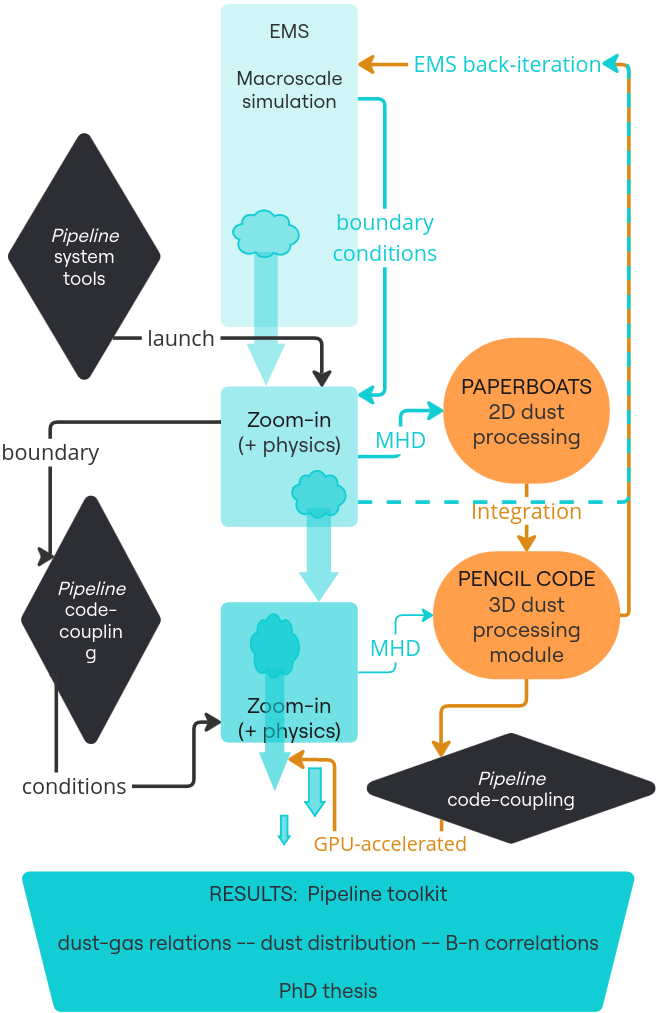
\includegraphics[trim=0.0cm 0.0cm 0.0cm 0.0cm, clip=true]{Pics/flowchart2.png}
 \begin{picture}(0,0)
    \put( -98,204){\footnotesize{$\mathcal{D}_0$}}
    \put(-105,124){\footnotesize{$\mathcal{D}_1$}}
    \put( -88, 81){\footnotesize{$\mathcal{D}_2$}}
    \put(-120, 42){\footnotesize{$\mathcal{D}_{n>2}$}}
    \put(-103,186){\tiny{$\mathcal{R}_1$}}
    \put( -90,123){\tiny{$\mathcal{R}_2$}}
    \put(-100, 86){\tiny{$\mathcal{R}_3$}}
  \end{picture}
    }
 \end{minipage}
\begin{minipage}[h]{0.59\textwidth}
\wpdef{2}{Dust}{Dust processing}
\textsc{Paperboats} shall be applied to new \textit{multi-scale} simulations over
a wider range of ISM environments, while being fully implemented into the
efficiently parallel sixth-order \textsc{Pencil Code} (PC).  Greater
acceleration shall be achieved by integration into the GPU-accelerated
\textsc{Pencil Code -- Astaroth} (PC-A) development with the Aalto
\href{https://www.aalto.fi/en/department-of-computer-science/hpclab}{\textbf{HPCLab}}. Code coupling of MHD and dust modeling will be developed to address
differences in timescales and computational load required for faster and more
efficient deployment of resources.
\tabto{0em}
Deliveries and expected results:
\tabto{0em}
$\bullet$~\textsc{Paperboats} implemented into highly scalable PC.
\tabto{0em}
$\bullet$~Dust modeling GPU-accelerated with PC-A.
\tabto{0em}
$\bullet$~Code-coupling tools: highly heterogeneous
codes or computations require resource management to avoid idle resources, match performance and reduce IO, memory or compute bottlenecks (\wpref{4} and \wpref{5}).
\end{minipage}
To implement \wpref{1} and \wpref{2} the PI has years of experience executing
such simulations with consistent success applying for resources on the Finnish
national infrastructure CSC, European infrastructure directly on LUMI, as well
as a member of successful HPCLab European scale PRACE projects.  Both the PI
and CoI also have continuous access to the National Academic Infrastructure for
Supercomputing in Sweden and, via our established US collaboration, to calls on
Frontier HPC resources.  Modifications to the dust modules and implementation
to PC-A are low risk, as the PI participates in the HPCLab development of the
PC-A implementation of SN driven turbulence, and partial dust-processing
modeling has successfully been implemented by the CoI.

\wpref{1} and \wpref{2} are assured results of high impact, since
they explore regimes of astrophysics with respect to dust distribution and
dynamics, magnetic field and ISM multi-phase structure, which are poorly
understood and important to observations and understanding of galaxy evolution.
Four publications are realistic, the rate and extent of any advances increasing
the better the success of \wpref{3} -- \wpref{5}.  The GS shall be included in
the execution and analysis of \wpref{1} and \wpref{2}, while their thesis shall
primarily address \wpref{3} and \wpref{4}.  New York and Ghent collaborators
have high expertise at modeling dust and MC.


%------------------------------------------------------------------------------
%------------------------------------------------------------------------------
\wpdef{3}{ODOP}{Pipeline -- ODOP tools}
\vspace{-0.3cm}
Data storage and management is commonly a bottleneck in any HPC, dealing with
datasets approaching TB and even PB scales. Scanning for regions of interest in
astrophysical simulations remains labour intensive and applied to disk-saved
datasets, output at intervals.  We shall apply cutting-edge machine-learning
tools for Opportunistic Data Operations \citep[][ODOP]{odop24} to analyze the
data to identify regions or patterns of interest and extract a suitable
subdomain from which to launch new experiments. Next these tools shall be
enhanced to work on active data in memory on-the-fly during the computation to
identify and extract relevant data when desired, and eventually launch such new
experiments.  This work is at the frontier of computer science, in which HPCLab
and \href{https://rdsea.github.io/}{\textbf{AaltoSEA}} are heavily
invested, and large-data use applications, such as this proposal are critical
for their development.
\tabto{0em}
Deliveries and expected results:
\tabto{0em}
$\bullet$ ODOP tools to identify critical patterns and extract relevant datasets.
\tabto{0em}
$\bullet$ Manage spawning EMS multi-scale simulations, rescheduling available resources to additional tasks and new physics, and .
\tabto{0em}
$\bullet$ Machine learning to manage additional resource requests and
execute new diagnostics.
%-----------------------------------------------------------------------------

%------------------------------------------------------------------------------
%------------------------------------------------------------------------------
\wpdef{4}{CC}{Pipeline -- code coupling}
\vspace{-0.3cm}
Defining consistent BCs after remeshing to macro-scale $\mathcal{D}_n$, without
erroneous artifacts in the flows, is a crucial step in the process.  Open
boundaries independent of $\mathcal{D}_{n-1}$ can work (paper in preparation),
but acquire only initial features from $\mathcal{D}_{n-1}$, which dissipate
over time.  Using surfaces from within $\mathcal{D}_{n-1}$ surrounding
$\mathcal{D}_n$ one may interpolate boundary values onto the fine grid (also in
time) to retain dynamically the macro-scale features.  High cadence slices from
$\mathcal{D}_{n-1}$ can be saved to disk and read subsequently for
$\mathcal{D}_{n}$ BC updates. Code-coupling on-the-fly, saves on storage, and
employs at the very least message passing interface (MPI).  Additional physics,
such as dust, cooling or self-gravity, necessitate diverging timescales or
computational load.  Code-coupling enhanced by machine learning could gain
speed by balancing load and available resources, by minimizing redundant
communication. The basic machinery for coupling multiple versions of the code
or with other codes would be similar.  HPCLab already has experience coupling
\textsc{Eulag} with \textsc{Pencil Code} (1-way).
\tabto{0em}
Deliveries and expected results:
\tabto{0em}
$\bullet$ Code-coupling to communicate BCs across multi-scales (1-way).
\tabto{0em}
$\bullet$ Code-coupling within multi-scale to balance computational load (2-way).
%------------------------------------------------------------------------------
%------------------------------------------------------------------------------

%-----------------------------------------------------------------------------
%-----------------------------------------------------------------------------
\begin{figure}[h]
    \begin{ganttchart}{1}{16}
      \gantttitle{Year 1}{4}
      \gantttitle{Year 2}{4}
      \gantttitle{Year 3}{4}
      \gantttitle{Year 4}{4} \\
%-----------------------------------------------------------------------------
      \ganttgroup{\wpref{1} (EMS)}{1}{15} \\
      \ganttbar{$R_1\rightarrow R_n$}{1}{3.5}
      \ganttbar{}{5}{7}
      \ganttbar{}{9}{11}
      \ganttbar{}{13}{15}\\
      \ganttmilestone[milestone/.append style={fill=blue!50}]{publications}{4}
      \ganttmilestone[milestone/.append style={fill=blue!50}]{}{8}
      \ganttmilestone[milestone/.append style={fill=blue!50}]{}{12}
      \ganttmilestone[milestone/.append style={fill=blue!50}]{}{16} \\
    \node (a) [fill=blue,draw,anchor=east] at ([xshift=4.6cm]current bounding box.0){MHD-Dust applications};
      \node (b) [fill=yellow,draw,anchor=west] at ([yshift=-0.8cm]a.west){Toolkit development};
      \node (c) [fill=green,draw,anchor=west] at ([yshift=-0.8cm]b.west){GPU-PC-Toolkit integration};
%-----------------------------------------------------------------------------
      \ganttgroup{\wpref{2} (Dust)}{1}{15} \\
      \ganttbar{\textsc{Paperboats}}{1}{3} \\
      \ganttmilestone[milestone/.append style={fill=blue}]{\textsc{Dust in PC}}{4} \\
      \ganttmilestone[milestone/.append style={fill=green}]{\textsc{Dust in PC-A}}{7} \\
      \ganttbar{\textsc{Pencil-code}}{5}{7}
      \ganttbar{}{9}{11}
      \ganttbar{}{13}{15}\\
%-----------------------------------------------------------------------------
      \ganttgroup[group/.append style={fill=yellow}]{\wpref{3} (ODOP)}{1}{4}
      \ganttgroup[group/.append style={fill=yellow}]{}{10}{15} \\
      \ganttbar[bar/.append style={fill=yellow}]{dev. ODOP selection}{1}{4} \\
      \ganttbar{ODOP applied}{5}{7} \\
      \ganttmilestone[milestone/.append style={fill=yellow!50}]{publication}{7} \\
      \ganttbar[bar/.append style={fill=yellow}]{ODOP coupling}{10}{12}
      \ganttbar{}{13}{15} \\
%-----------------------------------------------------------------------------
      \ganttgroup[group/.append style={fill=yellow}]{\wpref{3} (ODOP)}{1}{4}
      \ganttgroup[group/.append style={fill=yellow}]{}{10}{15} \\
      \ganttbar[bar/.append style={fill=yellow}]{dev. ODOP selection}{1}{4} \\
      \ganttbar{ODOP applied}{5}{7} \\
      \ganttmilestone[milestone/.append style={fill=yellow!50}]{publication}{7} \\
      \ganttbar[bar/.append style={fill=yellow}]{ODOP coupling}{10}{12}
      \ganttbar{}{13}{15} \\
      \ganttmilestone[milestone/.append style={fill=yellow!50}]{publication}{14} \\
%-----------------------------------------------------------------------------
      \ganttgroup[group/.append style={fill=yellow}]{\wpref{4} (Coupling)}{5}{12} \\
      \ganttbar[bar/.append style={fill=yellow}]{dev. coupling PC}{5}{7} \\
      \ganttbar{coupling applied}{9}{11} \\
      \ganttmilestone[milestone/.append style={fill=yellow!50}]{publication}{11} \\
%-----------------------------------------------------------------------------
      \ganttgroup[group/.append style={fill=green}]{\wpref{5} (GPU)}{5}{7}
      \ganttgroup[group/.append style={fill=green}]{}{9}{11}
      \ganttgroup[group/.append style={fill=green}]{}{13}{15} \\
      \ganttbar[bar/.append style={fill=green}]{dev. PC-A dust}{5}{7} \\
      \ganttbar{PC-A dust applied}{9}{11}
      \ganttbar{}{13}{15}
      \ganttvrule{}{4}
      \ganttvrule{}{8}
      \ganttvrule{}{12}
    \end{ganttchart}
    \vspace{-1.6em}
    \caption{
Gantt chart: proposed 4-yr timeline and \wpref{} organization. Blue denotes
science applications, results executed with PC and PC-A; yellow denotes
development and application of ODOP management tools; green denotes GPU
integration into PC and then into ODOP framework. At least 3 publications shall
have GS lead author, relevant to thesis; yellow to
\href{https://www.nature.com/natmachintell/}{\textbf{Nature Machine
Intelligence}} or
\href{https://ieeexplore.ieee.org/xpl/RecentIssue.jsp?punumber=9}{\textbf{IEEE
Transactions on Automatic Control}}; blue to
\href{https://www.nature.com/natastron/}{\textbf{Nature Astronomy}} or
\href{https://www.aanda.org/}{\textbf{Astronomy \& Astrophysics}}.}
    \label{fig:work-packages}
\end{figure}
%-----------------------------------------------------------------------------

\wpref{3} and \wpref{4} shall provide the framework around which the GS thesis
shall develop. Early in \wpref{3} the GS shall understand what manual
management is applied to the selection and management of data for \wpref{1} and
develop machine management tools to automate and learn these tasks using ODOP.
The GS with the support of the PI will implement code coupling (\wpref{4})
between versions of the PC or PC-A to handle differently loaded tasks while
communicating memory. This may extend to considering alternative uses of idle
central processors (CPUs) on GPU nodes and designing strategies applying to alternate types of
processing. Initial methods could rely on manual settings at executions, but
subsequently the focus shall return to \wpref{3} to implement run-time
ODOP-type control and responses to the code-coupling to maximize utilization and
reduce compute times. The support of collaborations in HPCLab and AaltoSEA and
the Aalto CS Doctoral program shall assist their Doctoral success.

%------------------------------------------------------------------------------
%------------------------------------------------------------------------------
\wpdef{5}{GPU}{GPU Acceleration}
\vspace{-0.3cm}
GPUs can offer a speed up 40--55$\times$ over traditional CPU
\citep{Astaroth22} and for applications much closer to the setup proposed here
the \textsc{Pencil Code -- Astaroth} (PC-A) yields speedup closer to 20$\times$
in our development tests.  This utilizes the higher functionality of
\textsc{Pencil Code} to compute and write diagnostics using idle CPUs while the
GPU solves the equations.  A simple speedup in this project is anticipated by
integrating \textsc{Paperboats} into PC-A.  Some operations are less efficient
on GPUs, such as solving FFTs. CPUs may therefore be better suited to solving
self-gravity. Code-coupling between GPU and CPU solvers, coupling nodes of
different type as required, shall be employed to distribute relevant
calculation tasks optimally and faster.
\tabto{0em}
Deliveries and expected results:
\tabto{0em}
$\bullet$~\textsc{Paperboats} implemented into highly scalable PC-A.
\tabto{0em}
$\bullet$ Code-coupling between GPU and CPU solvers.
%------------------------------------------------------------------------------
%------------------------------------------------------------------------------

The PI shall have responsibility for \wpref{5} and its integration within the
proposal, together with the HPCLab collaboration. This is an
extension of new physics to existing PC-A, which complements the outcomes in
\wpref{1} and \wpref{2}, which shall lead to a substantial speed up of the
calculations.

The Principal Investigator (PI) Maarit Korpi-Lagg\href{https://orcid.org/0000-0002-9614-2200}{
\includegraphics[scale=0.5]{orcid_16x16.jpeg}} \ldots
The Co-Investigator
(CoI) Frederick Gent\href{https://orcid.org/0000-0002-1331-2260}{
\includegraphics[scale=0.5]{orcid_16x16.jpeg}} has been
 a Research Fellow at the Aalto Computer Science Department until March 2025 and
 since November 2023 employed
as Assistant Professor at Nordita, Stockholm, under the five-year Swedish Research Council grant no. 2022-03767.
The responsibilities and research plan of the GS recruit shall match
their strengths and thesis goals best suited to the project.

The research environment at Aalto CS is highly conducive to success of the
project, with groups invested in HPC and machine learning tools, as well as an
international reputation for excellence in computer science.
\href{https://nordita.org/}{\textbf{Nordita}} (The Nordic Institute for
Theoretical Physics) also has international reputation for excellence in
astrophysics, and the CoI and PI are actively pursuing opportunities to further
enhance the Swedish funding for the joint project with the Swedish Space
Science Agency and foundations.  Finnish collaborations include
Prof.~Korpi-Lagg's
\href{https://www.aalto.fi/en/department-of-computer-science?check_logged_in=1}{\textbf{HPCLab}}
and Prof.~Truong's \href{https://rdsea.github.io/}{\textbf{AaltoSEA}} research
groups combining expertise in HPC, service engineering analytics of distributed
software systems, big data applications and machine learning tools.

%\vspace{-0.6cm}
\begin{tabular}{|m{4.0cm}|m{5.0cm}|m{7.0cm}|}
\hline
Collaborator & Institute & Role \\
\hline
\href{https://kirchschlager.github.io/}{{Lars Mattsson}}\href{https://orcid.org/0000-0003-2670-2513}{
\includegraphics[scale=0.5]{orcid_16x16.jpeg}} & Nordita \& Stockholm University & Modeling dust processing dynamics \\[0.1cm]
\href{https://kirchschlager.github.io/}{{Florian Kirchschlager}}\href{https://orcid.org/0000-0002-3036-0184}{
\includegraphics[scale=0.5]{orcid_16x16.jpeg}} & Ghent University & Modeling dust processing dynamics \\[0.1cm]
\href{https://TBA}{{??}}\href{https://orcid.org/0000-0000-0000-0000}{
\includegraphics[scale=0.5]{orcid_16x16.jpeg}} & Canada?? & Galaxy simulations?? \\[0.1cm]
\href{https://science.gsfc.nasa.gov/astrophysics/cosmology/bio/eliahu.dwek-1}{{Eli Dwek??}}\href{https://orcid.org/0000-0001-8033-1181}{
\includegraphics[scale=0.5]{orcid_16x16.jpeg}} & NASA Emeritus Professor & Supernova Remnants \& ISM and Dust \\[0.1cm]
\href{https://www.amnh.org/research/staff-directory/mordecai-mark-mac-low}{Mordecai-M Mac Low}\href{https://orcid.org/0000-0003-0064-4060}{
\includegraphics[scale=0.5]{orcid_16x16.jpeg}} & American Museum of Natural History, New York & Modeling astrophysical turbulence and physics of molecular clouds \\[0.4cm]
Hong-Linh Truong\href{https://orcid.org/0000-0003-1465-9722}{
\includegraphics[scale=0.5]{orcid_16x16.jpeg}} & Aalto University & analytics of distributed software systems, big data applications \& machine learning tools (ODOP)\\[0.4cm]
\hline
\end{tabular}
\vspace{-0.2cm}


\section{Responsible science}

\instructions{
This subsection is a mandatory part of the plan. All listed points must be fully addressed, as each constitutes a factor in the review and decision-making process. Furthermore, please note that applications will not be processed if any one of the following four elements is missing:
%
\begin{enumerate}
\item a description of dimensions related to gender equality and nondiscrimination in the research, or a justification if not relevant
\item a description of how equality and nondiscrimination will be promoted in the composition of the research group and collaborations
\item a description of how good scientific practice will be followed in the project
\item a description of how open access to research publications and research data will be ensured.
\end{enumerate}
\href{https://www.aka.fi/en/from-research-to-society/responsible-science/}{Read more about responsible science.}
%
	\begin{itemize}
		\item State whether dimensions related to gender equality and nondiscrimination are relevant to the proposed research
		\begin{itemize}
			\item If relevant, explain how these aspects are integrated into the research plan (e.g. concerning project’s objectives, methodology, analysis and dissemination)
			\item If not relevant, justify their non-applicability
		\end{itemize}
		\item Describe how equality and nondiscrimination will be promoted in the composition of the research group and collaborations
		\item Describe how good scientific practice will be followed in the project
		\item Explain how open access to research publications and research data will be ensured
		\item Consideration of sustainable development goals in project activities
	\end{itemize}
}

Insert your text here...

%------------------------------------------
%%%% REFERENCES %%%%
%The list of references is included in the length of the research plan. All references must be added directly into the text, for example as follows: (author(s), year) or [number]. You must not use footnotes. The list of references can be added manually or, for example, by using BibTeX.

\renewcommand\refname{References}


\bibliography{refs}% common bib file
%\begin{thebibliography}{5}
%\setlength{\parskip}{-6pt}
%% font size of references is 10 pt
%\footnotesize
%
%\bibitem{ref1}
	\instructions{The list of references is included in the length of the research plan. All references must be added directly into the text, for example as follows: (author(s), year) or [number]. You must not use footnotes. The list of references can be added manually or, for example, by using BibTeX. \\ \vspace{10pt}
Delete this instructions environment when preparing your text. \\ \vspace{10pt}}
%List the references here...
%
%\end{thebibliography}

%% Page counter for header
\label{lastpage}

\end{document}
